% Editable diagrams of the owner's two state-restricted truth examples.
% Build: make -C paper figure-trimmed-true-tree-v1
% Root depth is zero. Colored nodes, not whole shaded levels, are sampled.
% A: ((x,z)y,(v,u)u)u -> ((x,z)-,(u)u)u.
%    B_0 selects the internal right u. B_1 selects x and z.
% B: (((c,e)c)b,((d)d,(a)a)a)a -> (b,((d)d,(a)a)a)a.
%    B_0 selects b. B_1 selects the terminal right d and a.
% In these comments '-' denotes absence of a label, never a new state.
\documentclass[tikz,border=4pt]{standalone}
\usepackage[T1]{fontenc}
\usepackage{amsmath,amssymb}
\usetikzlibrary{arrows.meta,backgrounds}
\definecolor{CTBFnavy}{HTML}{27325E}
\definecolor{CTBFteal}{HTML}{2E7D78}
\definecolor{CTBForange}{HTML}{D8704A}
\begin{document}
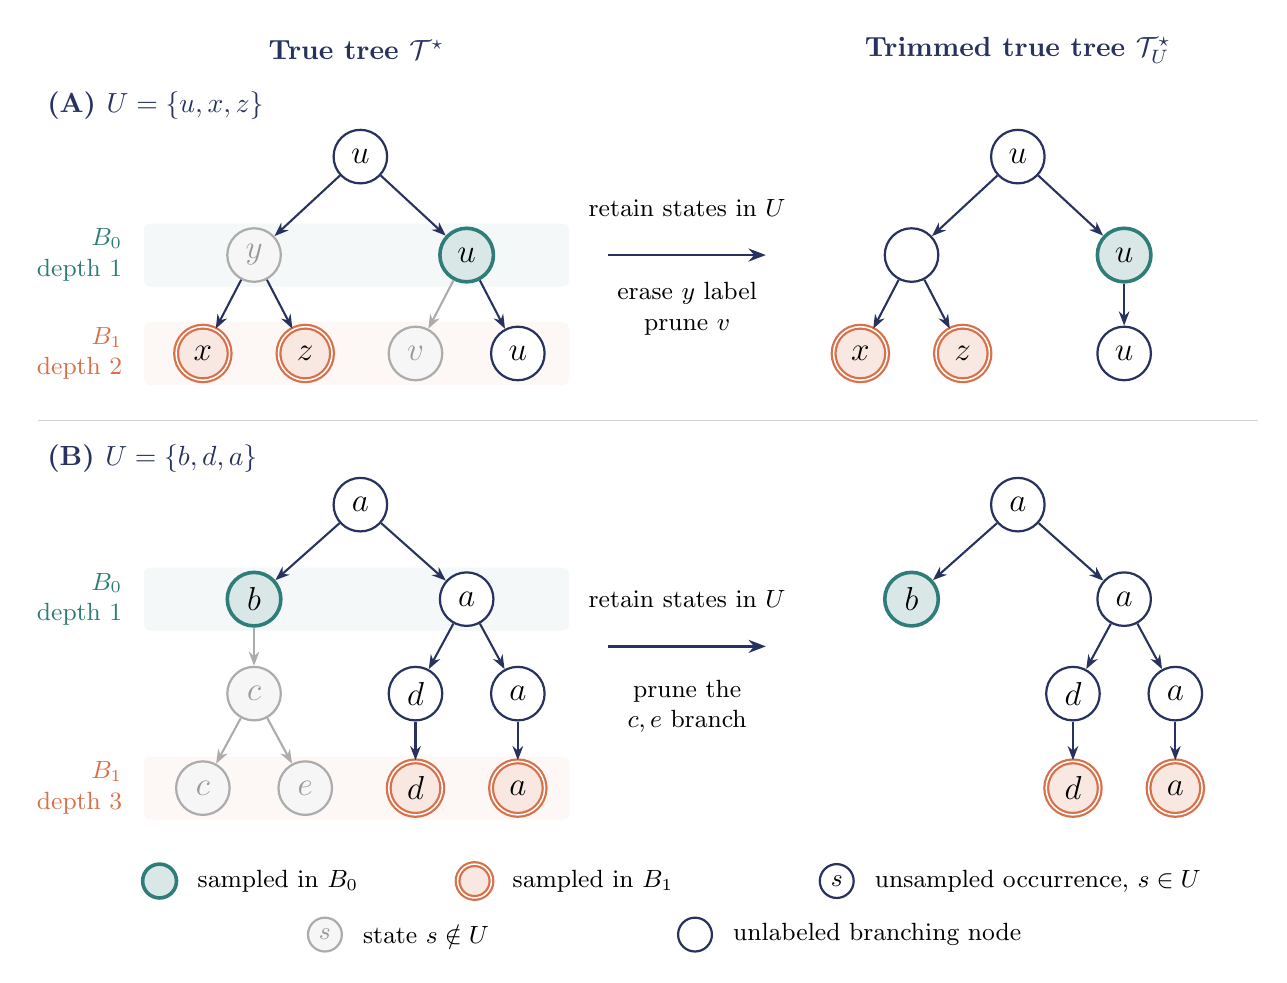
\begin{tikzpicture}[
  x=1cm,y=1cm,font=\sffamily,
  state/.style={circle,draw=CTBFnavy,fill=white,line width=.8pt,
    minimum size=6.8mm,inner sep=0pt,font=\large},
  early/.style={state,draw=CTBFteal,fill=CTBFteal!18,line width=1.3pt},
  late/.style={state,draw=CTBForange,fill=CTBForange!16,
    double=white,double distance=.55pt,line width=.8pt},
  outside/.style={state,draw=gray!65,text=gray!80,fill=gray!7},
  edge/.style={-{Stealth[length=1.8mm]},draw=CTBFnavy,line width=.75pt},
  excluded/.style={edge,draw=gray!65},
  reduction/.style={-{Stealth[length=2.2mm]},draw=CTBFnavy,line width=1pt},
  title/.style={font=\bfseries\normalsize,text=CTBFnavy},
  level/.style={font=\small,align=right,anchor=east},
  note/.style={font=\small,align=center}
]
\node[title] at (4.1,.15) {True tree $\mathcal T^\star$};
\node[title] at (12.5,.15) {Trimmed true tree $\mathcal T^\star_U$};

% Example A: all three u occurrences survive. The y vertex loses its label.
\node[title,anchor=west] at (.05,-.55) {(A) $U=\{u,x,z\}$};
\begin{scope}[on background layer]
  \fill[CTBFteal!5,rounded corners=2pt] (1.4,-2.85) rectangle (6.8,-2.05);
  \fill[CTBForange!5,rounded corners=2pt] (1.4,-4.1) rectangle (6.8,-3.3);
\end{scope}
\node[level,text=CTBFteal] at (1.25,-2.45) {$B_0$\\depth 1};
\node[level,text=CTBForange] at (1.25,-3.7) {$B_1$\\depth 2};

\node[state] (At-root) at (4.15,-1.2) {$u$};
\node[outside] (At-y) at (2.8,-2.45) {$y$};
\node[early] (At-u1) at (5.5,-2.45) {$u$};
\node[late] (At-x) at (2.15,-3.7) {$x$};
\node[late] (At-z) at (3.45,-3.7) {$z$};
\node[outside] (At-v) at (4.85,-3.7) {$v$};
\node[state] (At-u2) at (6.15,-3.7) {$u$};
\foreach \parent/\child in {At-root/At-y,At-root/At-u1,At-y/At-x,At-y/At-z,At-u1/At-u2}{
  \draw[edge] (\parent) -- (\child);
}
\draw[excluded] (At-u1) -- (At-v);

\node[state] (Ar-root) at (12.5,-1.2) {$u$};
\node[state] (Ar-y) at (11.15,-2.45) {};
\node[early] (Ar-u1) at (13.85,-2.45) {$u$};
\node[late] (Ar-x) at (10.5,-3.7) {$x$};
\node[late] (Ar-z) at (11.8,-3.7) {$z$};
\node[state] (Ar-u2) at (13.85,-3.7) {$u$};
\foreach \parent/\child in {Ar-root/Ar-y,Ar-root/Ar-u1,Ar-y/Ar-x,Ar-y/Ar-z,Ar-u1/Ar-u2}{
  \draw[edge] (\parent) -- (\child);
}
\draw[reduction] (7.3,-2.45) -- (9.3,-2.45);
\node[note] at (8.3,-1.85) {retain states in $U$};
\node[note] at (8.3,-3.13) {erase $y$ label\\prune $v$};

\draw[gray!35] (.05,-4.55) -- (15.55,-4.55);

% Example B: prune the c/e branch but preserve all a and d occurrences.
\node[title,anchor=west] at (.05,-5.03) {(B) $U=\{b,d,a\}$};
\begin{scope}[on background layer]
  \fill[CTBFteal!5,rounded corners=2pt] (1.4,-7.22) rectangle (6.8,-6.42);
  \fill[CTBForange!5,rounded corners=2pt] (1.4,-9.62) rectangle (6.8,-8.82);
\end{scope}
\node[level,text=CTBFteal] at (1.25,-6.82) {$B_0$\\depth 1};
\node[level,text=CTBForange] at (1.25,-9.22) {$B_1$\\depth 3};

\node[state] (Bt-root) at (4.15,-5.62) {$a$};
\node[early] (Bt-b) at (2.8,-6.82) {$b$};
\node[state] (Bt-a1) at (5.5,-6.82) {$a$};
\node[outside] (Bt-c1) at (2.8,-8.02) {$c$};
\node[state] (Bt-d1) at (4.85,-8.02) {$d$};
\node[state] (Bt-a2) at (6.15,-8.02) {$a$};
\node[outside] (Bt-c2) at (2.15,-9.22) {$c$};
\node[outside] (Bt-e) at (3.45,-9.22) {$e$};
\node[late] (Bt-d2) at (4.85,-9.22) {$d$};
\node[late] (Bt-a3) at (6.15,-9.22) {$a$};
\foreach \parent/\child in {Bt-root/Bt-b,Bt-root/Bt-a1,Bt-a1/Bt-d1,Bt-a1/Bt-a2,Bt-d1/Bt-d2,Bt-a2/Bt-a3}{
  \draw[edge] (\parent) -- (\child);
}
\foreach \parent/\child in {Bt-b/Bt-c1,Bt-c1/Bt-c2,Bt-c1/Bt-e}{
  \draw[excluded] (\parent) -- (\child);
}

\node[state] (Br-root) at (12.5,-5.62) {$a$};
\node[early] (Br-b) at (11.15,-6.82) {$b$};
\node[state] (Br-a1) at (13.85,-6.82) {$a$};
\node[state] (Br-d1) at (13.2,-8.02) {$d$};
\node[state] (Br-a2) at (14.5,-8.02) {$a$};
\node[late] (Br-d2) at (13.2,-9.22) {$d$};
\node[late] (Br-a3) at (14.5,-9.22) {$a$};
\foreach \parent/\child in {Br-root/Br-b,Br-root/Br-a1,Br-a1/Br-d1,Br-a1/Br-a2,Br-d1/Br-d2,Br-a2/Br-a3}{
  \draw[edge] (\parent) -- (\child);
}
\draw[reduction] (7.3,-7.42) -- (9.3,-7.42);
\node[note] at (8.3,-6.82) {retain states in $U$};
\node[note] at (8.3,-8.18) {prune the\\$c,e$ branch};

% Legend: color and border styles mark sampled occurrences, not state identity.
\node[early,minimum size=4.3mm] at (1.6,-10.4) {};
\node[font=\small,anchor=west] at (1.96,-10.4) {sampled in $B_0$};
\node[late,minimum size=4.3mm] at (5.6,-10.4) {};
\node[font=\small,anchor=west] at (5.96,-10.4) {sampled in $B_1$};
\node[state,minimum size=4.3mm,font=\small] at (10.2,-10.4) {$s$};
\node[font=\small,anchor=west] at (10.56,-10.4) {unsampled occurrence, $s\in U$};
\node[outside,minimum size=4.3mm,font=\small] at (3.7,-11.08) {$s$};
\node[font=\small,anchor=west] at (4.06,-11.08) {state $s\notin U$};
\node[state,minimum size=4.3mm] at (8.4,-11.08) {};
\node[font=\small,anchor=west] at (8.76,-11.08) {unlabeled branching node};
\end{tikzpicture}
\end{document}
